\documentclass[a4paper, 11pt]{article}

\usepackage[absolute]{textpos} % absolute positioned text blocks
\setlength{\TPHorizModule}{1mm}
\setlength{\TPVertModule}{1mm}
\usepackage[english]{babel}
\usepackage{csquotes}

% Images
\usepackage{graphicx} % used for images
\graphicspath{ {./../img/} }
\usepackage[labelfont=bf]{caption}

% Formatting
\usepackage{geometry} % better margins for document
\usepackage{titlesec} % better control over title spacing 
\usepackage{tabularx} % better tables
\usepackage[hidelinks]{hyperref} % hrefs
\usepackage{totcount}
\usepackage{pgfplots}
\pgfplotsset{compat=1.16}
\pgfplotsset{
    colormap={cool}{rgb255(0cm)=(237,66,76); rgb255(0.5cm)=(255,255,255); rgb255(1cm)=(57,146,239)}
}
\usepgfplotslibrary{colorbrewer}

\usepackage{float} % image placement
\usepackage{amssymb} % math symbols

% Code listings
\usepackage{listings}
\usepackage{commath}
\usepackage{pifont}
\usepackage{xcolor}
\definecolor{codered}{rgb}{0.93,0.26,0.298}
\definecolor{codegrey}{rgb}{0.7,0.7,0.7}
\definecolor{codepink}{rgb}{0.737,0.47,0.823}
\definecolor{codeblue}{rgb}{0.227,0.572,0.937}
\definecolor{codegreen}{rgb}{0.441,0.664,0.286}
\definecolor{codestring}{rgb}{0.58,0,0.82}
\definecolor{backcolor}{rgb}{0.95,0.95,0.95}
\definecolor{lightgrey}{rgb}{0.8,0.8,0.8}

\lstdefinelanguage{HLSL}{
	morekeywords=[1]{
        % variables
        seed,source,
	},
	morekeywords=[2]{
        % methods and functions
		getSeed,
	},
	morekeywords=[3]{
        % CONSTANTS
        INIT_SEED
    },
    keywordstyle=[1]\color{codeblue},
    keywordstyle=[2]\color{codered},
    keywordstyle=[3]\color{codepink},
	commentstyle=\color{codegrey},
	morestring=[b]", % defines that strings are enclosed in double quotes
	morestring=[b]', % defines that strings are enclosed in single quotes
    backgroundcolor=\color{backcolor},
    stringstyle=\color{codered},
    numberstyle=\tiny,
    basicstyle=\ttfamily\footnotesize,
    breakatwhitespace=false,
    breaklines=true,
    captionpos=b,
    keepspaces=true,
    numbers=left,
    numbersep=5pt,
    showspaces=false,
    showstringspaces=false,
    showtabs=false,
	tabsize=2,
    sensitive=false, % keywords are not case-sensitive
    morecomment=[l]{//}, % l is for line comment
    morecomment=[s]{/*}{*/}, % s is for start and end delimiter
    belowskip=2.5em,
    aboveskip=1em,
}

% Gantt charts
\usepackage{pgfgantt}

% drawings
\usepackage{tikz}
\usepackage{fontawesome}
\usetikzlibrary{positioning, shapes}
\usetikzlibrary{arrows.meta}
\geometry{
	a4paper,
	left=28mm,
	right=28mm,
    top=30mm,
    bottom=30mm
}

% Colors 
\RequirePackage{color}
\definecolor{bfhgrey}{rgb}{0.41,0.49,0.57}
\definecolor{brinkpink}{rgb}{1.0, 0.65, 0.79}
\definecolor{columbiablue}{rgb}{0.61, 0.87, 1.0}

% Glossary
\usepackage[toc]{glossaries}
\newacronym{gpu}{GPU}{ Graphics Processing Unit }
\newglossaryentry{latex}{name=LaTeX, description={ A high-quality document preparation system designed for the production of technical and scientific documentation }}

\makenoidxglossaries

\glsunset{gpu}

% Bibliography
\usepackage[backend=biber, style=ieee]{biblatex}
\addbibresource{partials/bibliography.bib}

\setcounter{secnumdepth}{3}
\titleformat{\paragraph}
{\normalfont\normalsize\bfseries}{\theparagraph}{1em}{}
\titlespacing*{\paragraph}
{0pt}{3.25ex plus 1ex minus .2ex}{1.5ex plus .2ex}

\begin{document}

\color{black}

\title{\doctitle}
\author{\docauthor}
\date{\versiondate}

\newcounter{requirements}
\newtotcounter{versionnumber}
\newcommand{\docsubtitle}{Project documentation}
\newcommand{\docauthor}{Matthias Thomann}
\newcommand{\doctitle}{Strong Entropy Sources for Randomness Extractors}
\newcommand{\fieldofstudies}{BSc in Computer Science}
\newcommand{\specialisation}{Computer perception and virtual reality}
\newcommand{\prof}{Prof. Dr. Rolf Haenni}

\newcommand{\versiondate}{\today}
\newcommand{\sectionref}[1]{\autoref{#1}}
\newcommand{\emptyline}{\vspace{\baselineskip}\\\noindent}

\titlespacing*{\section} {0pt}{7.5ex plus 1ex minus .2ex}{2.3ex plus .2ex}
\titlespacing*{\subsection} {0pt}{4.25ex plus 1ex minus .2ex}{1.5ex plus .2ex}

\pagenumbering{roman}
\setcounter{page}{3}

%% include BFH logo and HuCE-ml logo

\begin{titlepage}

\setlength{\unitlength}{1mm}

\begin{textblock}{20}[0,0](22,12)
    
\includegraphics{BFH_Logo_B.png}
\end{textblock}

\begin{flushleft}

\vspace*{21mm}

\fontsize{24.88pt}{40pt}\selectfont
\textbf{\doctitle}
\vspace{2mm}

\fontsize{17.28pt}{24pt}\selectfont\vspace{0.3em}
\docsubtitle
\vspace{1cm}

% \begin{figure}[H]
%     \centering
%     \includegraphics[width=\linewidth]{unity captures/final_dusk.PNG}
% \end{figure}

\fontsize{10pt}{12pt}\selectfont
\begin{textblock}{150}(28,225)
\fontsize{10pt}{17pt}
\begin{tabbing}
xxxxxxxxxxxxxxxxxxxxx\=xxxxxxxxxxxxxxxxxxxxxxxxxxxxxxxxxxxxxxxxxxxxxxx \kill
Field of Studies:	\> \fieldofstudies	\\
Specialization:	    \> \specialisation	\\
Author:		        \> \docauthor \\
Supervisor:         \> \prof \\
Date:			    \> \versiondate \\
Version:		    \> 1.0 \\
\end{tabbing}

\end{textblock}

\begin{textblock}{150}(28,280)
\noindent 
\color{bfhgrey}\fontsize{9pt}{10pt}\selectfont
Berner Fachhochschule | Haute \'ecole sp\'ecialis\'ee bernoise | Bern University of Applied Sciences
\color{black}\selectfont
\end{textblock}

\end{flushleft}

\end{titlepage}
\clearpage

\section*{Abstract}
This is an abstract.
\clearpage

\tableofcontents
\clearpage

\pagenumbering{arabic}

\section{General}

\subsection{Purpose}
During this project, all gathered information and knowledge about the researched algorithms and techniques are written down. All prototypes and the final results are documented and compared with real photographs of clouds.

\subsection{Audience}
This document is written with the intent to further expand existing knowledge about the topic, hence it requires a fundamental knowledge about computer graphics and rendering.

\subsection{Revision History}
\begin{tabularx}{\textwidth}{|l|l|c|X|}
    \hline
    \textbf{Version}         & \textbf{Date}     & \textbf{Name}     & \textbf{Comment}                  \\ \hline \addtocounter{versionnumber}{1}
    0.\arabic{versionnumber} & March 21, 2020    & Matthias Thomann  & Initial draft                     \\ \hline
\end{tabularx}
\clearpage

\section{Entropy Sources}

The concept of information theory is that the \emph{informational value} of any given message is defined by how much content of it is deemed as surprising. Therefore, the entropy source is described as to where the message originated from.
\newline
In a more technical manner, one has to understand that algorithms and protocols that work with randomness are assuming that the computer has access to a sequence of truly random bits.
Shaltiel describes those as a sequence of independent and unbiased coin tosses\cite{randomness:extractor2}.
Of course, in actual implementations this sequence is generated by taking a sample from some “source of randomness”, also known as an \emph{entropy source}.

\subsection{Quantifying Unpredictability}
\label{entropy:quantifying}
First, in order to be able to determine how weak or strong an entropy source is, one has to define how unpredictable the source is.
But as described by Kelsey\cite{entropy1}, there are some issues when it comes to quantifying unpredictability. 
For example, a series of coin flips is not reliable enough as there is insufficient information. Another example might be that the intended source is too complex to model.
\newline
However, there is a way to determine how reliable a source really is, which is calculating the entropy. There are several approaches to this issue.

\subsubsection{Shannon-Entropy}
\label{shannon}
Conceptually, information can be thought of as being stored in variables that can take on different values.
The entropy of a variable is the amount of information contained in the variable.
It is not quantified by the number of different values it can take on or its length, but rather how much of the information is new.
This quantification of information is called the \emph{Shannon entropy}. It is formally defined as:
\begin{equation}
    E = -\sum\limits_{i=1}^k p(i) \times \log_2 p(i)
\end{equation}

\noindent
To put the equation in an example, it is best to think of a fair coin that is flipped twice in a row. The chances for each result are as follows:
\begin{itemize}
    \item $p_1 = p(\text{heads once, tails once}) = 0.25 + 0.25 = 0.5$
    \item $p_2 = p(\text{heads twice}) = 0.5 \times 0.5 = 0.25$
    \item $p_3 = p(\text{tails twice}) = 0.5 \times 0.5 = 0.25$
\end{itemize}

\noindent
So for $p_1$, the entropy would be $0.5 \times \log_2 0.5 = 0.5 \times -1 = -0.5$.
For both $p_2$ and $p_3$, it is $0.25 \times \log_2 0.25 = 0.25 \times -2 = -0.5$.
\newline
So in total, $E = -\left( p_1 + p_2 + p_3 \right) = 1.5$. The Shannon entropy $E$ of the example above is therefore denoted as 1.5 \emph{bits} or \emph{shannons}.


\subsubsection{Min-Entropy}
Next to the famous Shannon entropy, other well known formulas have been developed. 
The so-called \emph{min-entropy} is the most conservative way of measuring the unpredictability of a set of outcomes. It is defined as follows, where $H$ is the entropy and $p$ is the probability of each event:
\begin{equation}
    H = -\log_2 \underset{1 \le i\le k}{max} \left(p_i\right)
\end{equation}
\noindent
Generally, it is recommended to work with the min-entropy as it represents a very conservative measure of entropy.
It is based solely on the biggest probability. Therefore, it is measuring the effectiveness of the strategy of guessing the most likely output of the entropy source\cite{randomness:sources2}.
\newline
For the example in \sectionref{shannon}, the min-entropy $H$ would be calculated as follows, as $p_1$ is the biggest probability:
\begin{equation}
    H = -\log_2 \left(p_1\right) = -\log_2 0.5 = 1\,bit
\end{equation}

\noindent
Note that the maximum possible value for the min-entropy of a random variable with $k$ distinct values is $\log_2 k$, which is the case when the random variable $X$ has a uniform probability distribution, like $p_1 = p_2 = ... = p_k = 1/k$.

\clearpage
\subsection{Real-Life Uses}
Naturally, there are different kind of sources, each with individual strength in terms of the quality of randomness.
This model shows the entropy source in detail. Each component will now be explained further.

\begin{figure}[H]
    \centering
    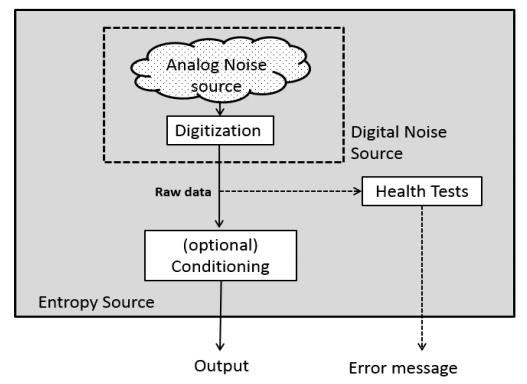
\includegraphics[width=\linewidth]{entropy-source.PNG}
    \caption{Depiction of an entropy source model \cite{randomness:sources1}.}
\end{figure}

\subsubsection{Practical examples}
Some practical examples of entropy sources are 

\begin{itemize}
    \item Measuring user dependent behavior, for example mouse movement or keyboard stroke timings.
    \item Measuring timing of past events, for example how much time the last disk operation took.
    \item Measuring thermal or radioactive noise.
    \item Measuring voltage levels.
\end{itemize}

\noindent
More interestingly, here are the sources that are typically able to be access in software, repeating some of the above:

\begin{itemize}
    \item Timings between key presses
    \item Timings and positions of mouse movements
    \item Timings between interrupts and related events, such as packets arriving to a network card, data arriving from a disk controller...
    \item Timings at which successive threads are scheduled on to the processor
    \item The amount of free memory
    \item Details of files that are liable to change frequently, for example the contents of the "temp" directory
    \item System temperature monitor readings
    \item Noise like a microphone input or other peripherals, for example a video camera
\end{itemize}
\subsection{Measuring and Digitizing}
It is important to note that the entropy source has the be measured and digitized in order for the randomness extractor to use it.
This, of course, can prove to be difficult in some cases where one does not have access to any kind of proper measurement tools.

\subsubsection{Quality}
As mentioned above, sampling the entropy source can introduce errors. It also provokes the question whether or not the user is measuring what he/she thinks that he/she is actually measuring.
One factor could be the noise or unreliability of readings produced by the measuring unit. Another question to solve is how much o sample variability is entropy and how much is just the complexity of the model.
\newline
To counter at least some model problems, the sampling rate can be adjusted. For example, measuring voltage level or thermal noise with frequency that is too high, correlated outputs are produced.
This can be fixed by decreasing the rate at which the source is measured.

\subsubsection{Performance}
Equally important as the quality of the measurement of an entropy source is the performance of the measurement. Understandably, electronic systems tend to be the fastest. An example of slower events are loading executions of the operating system and system level events.
Even slower are simple physical events, like the interactions between humans and computers.

\subsubsection{Additional Noise Sources}
As it may happen, other additional sources of noise may be available to the system of the entropy source's origin.
Understandably, outputs of those additional sources may be combined to form a joint entropy of the outputs across all sources.
However, it may prove to be hard to estimate the entropy of the combined sources. Also, dependencies between those sources may further complicate the entropy estimation.
\newline
Furthermore, it is assumed that the entropy sources have a unique primary noise source that is responsible to generate randomness. 
The National Institute of Standards and Technology (NIST) describes the issue as follows: "It should be noted that multiple copies of the same physical noise source are considered as a single noise source (e.g., a source with eight ring
oscillators, where the sampled bits are concatenated to get an eight-bit output, or where the samples bits are XORed together)" \cite{randomness:sources1}.

\subsection{Validation}
Entropy source validation is a necessary step in the process in order to obtain assurance that all relevant requirements are met.
There are established programs to validate any given entropy source officially. 
The National Voluntary Laboratory Accreditation Program (NVLAP) is a program by the NIST specifically for testing, calibrating and accrediting laboratories.
The Cryptographic Algorithm Validation Program (CAVP) and Cryptographic Module Validation Program (CMVP) both provide reviews of the results\cite{entropy:cmvp}.
\newline
Validation provides additional assurance that adequate entropy is provided by the
source and may be necessary to satisfy some legal restrictions, policies, and/or directives of various
organizations.
\newline
As described by Kelsey et al. \cite{randomness:sources1}, the validation consists of testing by an NVLAP-accredited
laboratory against the requirements of SP 800-90B, followed by a review of the results by CAVP and CMVP.
The SP 800-90B is a recommendation by NIST for the entropy sources used for random bit generation\cite{entropy:validation}.

\subsubsection{Validation Process}
First of all, there are restrictions and requirements for the submitted data, which is to be validated.
A sequential dataset of at 1'000'000 sample values obtained directly from the noise source is necessary.
Should it not be possible to obtain that many samples, it is also allowed to use a concatenation of several smaller sets of consecutive samples.
\newline
The validation process defined by NIST also speaks of a \emph{conditioning component} (see \sectionref{conditioning}).
If such a component was used, another 1'000'000 consecutive conditioning component outputs must be submitted, concatenated in order they were generated and treated as a binary string for testing purposes.
\emptyline
For the validation process, an entropy estimate has to by submitted next to the sample data. 
The entropy estimate of a noise source, which is calculated from a single, long-output sequence, might
provide an overestimate if the noise source generates correlated sequences after restarts. 
This is why the source is restarted during validation exactly 1'000 times. Each time, a set of 1'000 consecutive samples from the source are collected and an output is generated.
\newline
Usually, a restart of the entropy source could be as simple as powering off the system, letting it cool down, wait for ten seconds, then proceed.
\newline
The idea behind those restart tests is to re-evaluate the entropy estimate that was provided for the entropy source, by using different outputs from many restarts. Additionally, it ensures that the outputs, generated after a restart, are drawn from the same distribution as every other output.
It is important to note that the tests will also reveal whether or not the distribution of samples in a restart sequence is independent of its position in the restart sequence.

\subsection{Health Tests}
The validation is an official process that is required to check if the entropy source does provide enough entropy.
But what if the entropy source is erroneous? This is where \emph{health tests} are introduced, a vital and required part of any entropy source.
\newline
They aim to detect deviations from the intended behavior of the noise source in a quick and efficient manner.
Also, they should be able to provide a high chance of correct assessments.
A health test works by taking the output of the entropy source as input and characterizing the expected behavior based on those values.
\emptyline
Health tests are necessary as entropy sources may be fragile. Examples of how an entropy source could be influenced are mainly physical conditions of the device in use, such as:
\begin{itemize}
    \item Temperature
    \item Humidity
    \item Electric field
\end{itemize}

\subsubsection{Deviation Detection}
Naturally, the questions arises as how to detect if an entropy source is actually healthy and stable.
For that, there are multiple ways of doing so. In the publication of the SP 800-90B recommendation by NIST\cite{randomness:sources1}, common occurrences are:
\begin{enumerate}
\item When there is a significant decrease in the entropy of the outputs
\item When noise source failures occur
\item When hardware fails, and implementations do not work correctly
\end{enumerate}

\subsubsection{Types of Health Tests}
An important detail to note is that health tests are performed before any conditioning (see \sectionref{conditioning}) is done.
Also, there are different types of health tests. In a similar fashion to the restart tests, \emph{start-up health tests} are applied after the system has been started or restarted, before the first use of the entropy source.
They specifically validate that nothing has failed since the last use of the entropy source .
\newline
Then there are \emph{continuous health tests}. These are run, as the name suggests, continuously and indefinitely on the outputs of the entropy source. Their goal is to detect failures during the use of the source, as it produces outputs.
The continuous health tests use the digitized output of the underlying source and since they are executed constantly, it is important for them to have an extremely low chance of raising a false alarm.
Since one can assume that the device has a low false positive probability itself, health tests are generally designed to mainly detect bigger failures.
\newline
In some cases, in order for the health test to be able to detect failures, it has to accumulate data over time.
Should a failure be detected during usage of an entropy source, one has to assume that some or most of the past outputs may be subject to error due to an erroneous source or failure in the source.
\newline
Lastly, NIST defined \emph{on-demand health tests} as tests that can be called at any time.
They are usually not required to be executed during operation. However, the entropy source must be capable of performing such tests during runtime.
\emptyline
Should an error arise or should the health test detect a failure, it is job of the entropy source to notify the consuming application.

\subsection{Entropy Estimation}
It is already established that a strong entropy source is one that has the ability to reliably create random outputs.
In \sectionref{entropy:quantifying}, a way of how to calculate the entropy of any given entropy source was introduced.
In practice, there are more methods than just using the min-entropy.

\subsubsection{Independent and Identically Distributed}
The samples from a noise source are \emph{independent and identically distributed} (IID) if each sample
has the same probability distribution as every other sample, and all samples are mutually
independent, as it is described by NIST\cite{randomness:sources1}.
Since a reliable entropy source should not be identically distributed, this is not the desired case. Also, a viable entropy source fails to produce IID outputs.

\subsubsection{Recommended Estimators}
The method used to estimate the entropy of an entropy source is called an \emph{estimator}. Usually, it is recommended to use an estimated named "The Most Common Value Estimator", better known as the min-entropy estimator.
\newline
If the output of an entropy source is IID, is it recommended to only use the min-entropy estimator to calculate the entropy, as the entropy source is weak and therefore, only a very conservative way of measuring entropy should be used.
\emptyline
For non-IID data, many different estimators can be applied to the outputs in order to calculate the entropy. Only to name a few, there is the collision estimator, the Markov estimator, the compression estimator and many more.
However, this document will not go deeper into the details of each different estimator.


\subsection{Conditioning Component}
\label{conditioning}
In the process of random number generation, a so-called \emph{conditioning component} may be used.
As previously described, the higher the entropy of a noise source, the better, as it reflects the unpredictability of the source.
Therefore, if a source has too many outputs, a conditioning component may be used to reduce the bias\cite{randomness:generation1}.
\begin{figure}[H]
    \centering
    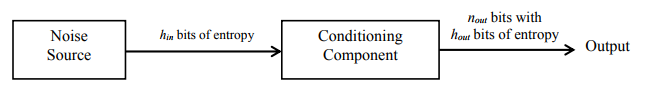
\includegraphics[width=\linewidth]{conditioning.png}
    \caption{Conditioning component used on an entropy source\cite{randomness:sources1}.}
\end{figure}

% \noindent
% TODO It is defined as follows:
\clearpage

% DUMMY ENTRIES, REMOVE WHEN GLOSSARY OR REFERENCES ARE ACTUALLY USED.
\nocite{gitlab}
\gls{gpu}
% REMOVE

\printnoidxglossary 
\clearpage
\printbibliography[heading=bibintoc]
\clearpage
\phantomsection
\addcontentsline{toc}{section}{Listings}
\phantomsection
\addcontentsline{toc}{subsection}{Figures}
\listoffigures
\clearpage
\phantomsection
\addcontentsline{toc}{subsection}{Code Listings}
\lstlistoflistings

\end{document}
